\documentclass[a4paper,11pt,oneside]{book}

%%% το αρχείο αυτό καθορίζει το look που έχουν οι pythonies
%%% γίνεται \input από όλα τα κεφάλαια και τα φύλλα εργασίας

% χρησιμοποιούμενα πακέτα: 
% 
% polyglossia
% xstring
% graphicx
% caption
% xcolor
% hyperref
% minted
% geometry
% titlesec
% datetime
% changepage
% ntheorem

% οριζόμενες εντολές:
%
% smallcaps (βοηθ. removeaccents)
%    μικρά κεφαλαία χωρίς τόνους στα φωνήεντα
% scaling
%    η κλιμάκωση *όλων* των illustrations, τρέχουσα τιμή 0.9
% iconcomputer, iconkeyboard, icondiscuss, iconfillin, iconcaution, iconprompt, dottedline
%    εικονίδια για τα φύλλα εργασίας και εστιγμένη γραμμή
% marginnote
%    πλευρικό σχόλιο
% chapterwabstract (βοηθ. abstract, boxcolor, chaptercolor, concepts, tmpconcepts)
%    εισαγωγικό κείμενο κεφαλαίου με χρωματιστό τετράγωνο, συνοδευτικές έννοιες, κλπ.
% tobecontinued
%    εμφανίζει το "συνεχίζεται στην επόμενη σελίδα"

% οριζόμενα περιβάλλοντα:
% 
% note
%    μια υποσημείωση ή υπόδειξη, με μικρότερα γράμματα
% question
%    μια ερώτηση που "οδηγεί" κάθε νέα ενότητα
% answer
%    μια απάντηση σε μια ερώτηση του φύλλου εργασίας
% theory
%    μια ενότητα "θεωρίας" (στο τέλος ενός κεφαλαίου)
% exercise
%    μια αριθμημένη άσκηση
% step
%    ένα αριθμημένο βήμα (για φύλλο εργασίας)

% για μορφοποίηση κώδικα:
%
% pycode (περιβάλλον)
%     κώδικας python χωρίς αρίθμηση
% pyfile (εντολή)
%     εισαγωγή κώδικα python από αρχείο
% pyfilenl (εντολή)
%     εισαγωγή κώδικα python από αρχείο χωρίς αρίθμηση γραμμών
% pyfilesrc (εντολή)
%    εισαγωγή κώδικα από αρχείο με link στο αρχείο
% pyinline (εντολή)
%     κώδικας python μέσα στη ροή του κειμένου
% pyplain (περιβάλλον, για τα φύλλα εργασίας)
%     κώδικας python χωρίς φόντο
% pynew (περιβάλλον, για τα φύλλα εργασίας)
%     κώδικας python με φόντο
% pyterm (περιβάλλον για τα φύλλα εργασίας)
%     η είσοδος του χρήστη ή τα περιεχόμενα της οθόνης
% pyhighlight (εντολή)
%    highlight κειμένου (χρησιμοποιείται για κώδικα μέσα σε pyplain)


%%% επιλογές γλώσσας και γραμματοσειρών για το XeLaTeX

\usepackage{polyglossia}
\setdefaultlanguage{greek}
\setmainfont[Ligatures=TeX,SmallCapsFont={Linux Libertine O C},SmallCapsFeatures={Letters=SmallCaps}]{Linux Libertine O}
\setsansfont{Linux Biolinum O}
\setmonofont{Ubuntu Mono}
\enablehyphenation

% αφαίρεση τόνων από τα smallcaps
\usepackage{xstring}
\newcommand{\removeaccents}[1]{%
\def\result{#1}%
\StrSubstitute{\result}{ά}{α}[\result]%
\StrSubstitute{\result}{έ}{ε}[\result]%
\StrSubstitute{\result}{ή}{η}[\result]%
\StrSubstitute{\result}{ί}{ι}[\result]%
\StrSubstitute{\result}{ό}{ο}[\result]%
\StrSubstitute{\result}{ύ}{υ}[\result]%
\StrSubstitute{\result}{ώ}{ω}[\result]%
\StrSubstitute{\result}{Ά}{Α}[\result]%
\StrSubstitute{\result}{Έ}{Ε}[\result]%
\StrSubstitute{\result}{Ή}{Η}[\result]%
\StrSubstitute{\result}{Ί}{Ι}[\result]%
\StrSubstitute{\result}{Ό}{Ο}[\result]%
\StrSubstitute{\result}{Ύ}{Υ}[\result]%
\StrSubstitute{\result}{Ώ}{Ω}[\result]%
\result
}

\newcommand{\smallcaps}[1]{\textsc{\removeaccents{#1}}}

%%% εικόνες και λεζάντες

\usepackage{graphicx}
\newcommand{\scaling}{0.9}
\usepackage{caption}
\captionsetup{font=footnotesize}

%%% ειδικά περιβάλλοντα

\usepackage{xcolor}

% ερωτήσεις (που οδηγούν στην επόμενη ενότητα)
\definecolor{questioncolor}{rgb}{0.6,0.5,0.5}
\newenvironment{question}{\noindent\itshape\color{questioncolor}}{\noindent\ignorespaces}

% απαντήσεις (για τις ερωτήσεις των φύλλων εργασίας)
\definecolor{answercolor}{rgb}{0.5,0.5,0.5}
\newenvironment{answer}{\marginnote[16pt]{\iconfillin}\noindent\itshape\color{answercolor}}{\noindent\ignorespaces}

% περιβάλλον "θεωρίας" (πλήρες πλάτος κειμένου)
\usepackage{changepage}
\newenvironment{theory}[1]{\begin{adjustwidth}{}{-\overhang}\smallcaps{#1}\itshape}{\end{adjustwidth}}

% απομεινάρια...
% \newlength{\theoryrulelength}
% \setlength{\theoryrulelength}{36pt}
% \newenvironment{theory}{\rule{\theoryrulelength}{0.4pt}\begin{adjustwidth}{}{-\overhang}\itshape}{\end{adjustwidth}\rule{\theoryrulelength}{0.4pt}}

%%% υπερσύνδεσμοι

\definecolor{linkcolor}{rgb}{0.0,0.5,0.25}
\usepackage[colorlinks=true,urlcolor=linkcolor]{hyperref}

%%% εικονίδια και εστιγμένες γραμμές (για τα φύλλα εργασίας)

\newcommand{\iconcomputer}{
\includegraphics[scale=0.35]{../../share/circle-icons/one-color/computer.eps}}
\newcommand{\iconkeyboard}{
\includegraphics[scale=0.35]{../../share/circle-icons/one-color/keyboard.eps}}
\newcommand{\icondiscuss}{
\includegraphics[scale=0.35]{../../share/circle-icons/one-color/chat.eps}}
\newcommand{\iconfillin}{
\includegraphics[scale=0.35]{../../share/circle-icons/one-color/compose.eps}}
\newcommand{\iconcaution}{
\includegraphics[scale=0.35]{../../share/circle-icons/one-color/caution.eps}}
\newcommand{\iconprompt}{
\includegraphics[scale=0.35]{../../share/circle-icons/one-color/prompt.eps}}
\newcommand{\dottedline}{\vspace{\parskip}\dotfill}

%%% συνεχίζεται στην επόμενη σελίδα

\newcommand{\tobecontinued}{\mbox{}\hfill{\footnotesize ...συνεχίζεται στην επόμενη σελίδα.}}
\newenvironment{note}{\small\upshape}{}

%%% μορφοποίηση κώδικα με το pygmentize

\usepackage{minted}

% fix για ένα bug στο minted που εμφανίζεται όταν χρησιμοποιείται χρώμα στο φόντο (bgcolor)
% http://tex.stackexchange.com/questions/228058/how-to-space-before-and-after-a-minted-code-block-with-bgcolor
\makeatletter
\patchcmd{\minted@colorbg}{\noindent}{\noindent}{}{}
\apptocmd{\endminted@colorbg}{}{}{}
\makeatother

% χρώματα φόντου για τον κώδικα
\definecolor{codebg}{rgb}{0.80,0.95,0.85}
\definecolor{newcodebg}{rgb}{0.75,0.95,0.85}

% ορισμοί για τα περιβάλλοντα κώδικα
% pycode: περιβάλλον κώδικα python χωρίς αρίθμηση
\newminted[pycode]{python3}{bgcolor=codebg}
% pyfile: python από αρχείο
\newmintedfile[pyfile]{python3}{linenos=true,numberblanklines=false,escapeinside=||,bgcolor=codebg}
% pyfilenl: python από αρχείο χωρίς αρίθμηση γραμμών
\newmintedfile[pyfilenl]{python3}{linenos=false,numberblanklines=false,escapeinside=||,bgcolor=codebg}
% pyinline: python μέσα στη ροή του κειμένου
\newmintinline[pyinline]{python3}{linenos=true,numberblanklines=false}
% pyplain: (για τα φύλλα εργασίας) περιβάλλον χωρίς φόντο
\newminted[pyplain]{python3}{bgcolor=white,escapeinside=||,formatcom={\upshape}}
% pynew: (για τα φύλλα εργασίας) περιβάλλον με φόντο
\newminted[pynew]{python3}{bgcolor=newcodebg,escapeinside=||,formatcom={\upshape}}
% pyterm: (για τα φύλλα εργασίας) περιβάλλον για τα περιεχόμενα της οθόνης
\newminted[pyterm]{text}{bgcolor=white,escapeinside=||}

%\newminted[pyterm]{text}{escapeinside=||}
% [TODO] fix: το pyterm χωρίς bgcolor εμφανίζει μεγαλύτερα περιθώρια (πάνω και κάτω) και δεν φαίνεται ωραίο. Το bgcolor είναι προσωρινό workaround, έχει κι αυτό margins (για να μην είναι κολλητά ο κώδικας με το περιθώριο) κι έτσι ο κώδικας στ' αριστερά δεν είναι τέλεια στοιχισμένος.

% εντολή για κώδικα από αρχείο με link στο αρχείο
\newcommand{\pyfilesrc}[2][]{%
\pyfile[#1]{#2}\\
\mbox{}\hfill{\scriptsize\href{http://pythonies.mysch.gr/#2}{\url{#2}}}
}

% εντολή για το highlighting του κώδικα (συνήθως σε pyplain περιβάλλον με escapeinside)
\newcommand{\pyhighlight}[1]{\colorbox{newcodebg}{#1}}

%%% αριθμημένα περιβάλλοντα

\usepackage{ntheorem}

% άσκηση
\makeatletter
\theoremheaderfont{\upshape}%\upshape\bfseries\scshape}
\theorembodyfont{\itshape}%\slshape}
\newtheoremstyle{lmargin}%
  {\item[\theorem@headerfont \llap{##2}\hskip\labelsep\hskip-6pt]}%
  {\item[\theorem@headerfont \llap{##2}\hskip\labelsep ##1\ (##3)\theorem@separator]}
\makeatother
\theoremstyle{lmargin}
\newtheorem{exercise}{}[chapter]

% βήμα φύλλου εργασίας
\makeatletter
\theoremheaderfont{\bfseries}%\upshape\bfseries\scshape}
\theorembodyfont{\upshape}%\slshape}
\newtheoremstyle{lmarginup}%
  {\item[\theorem@headerfont \llap{##2}\hskip\labelsep\hskip-6pt]}%
  {\item[\theorem@headerfont \llap{##2}\hskip\labelsep ##1\ (##3)\theorem@separator]}
\newtheoremstyle{slmarginup}%
  {\item[\theorem@headerfont \llap{##1##2.}\hskip\labelsep\hskip-6pt]}%
  {\item[\theorem@headerfont \llap{##2.}\hskip\labelsep ##1\ (##3)\theorem@separator]}
\makeatother

% deprecated: \newcommand{\standalone}{} to define standalone
%\ifdefined\standalone
    \theoremstyle{slmarginup}
    \newtheorem{step}{}
%\else
%    \theoremstyle{lmarginup}
%    \newtheorem{step}{}[chapter]
%\fi

%%% γεωμετρία σελίδας και συναφείς ορισμοί από το tufte-latex
%%% https://tufte-latex.github.io/tufte-latex/

% εσοχή και διάστημα μεταξύ παραγράφων
% δεν επηρρεάζει το tufte-latex
\parindent=0pt
\parskip=6pt

% γεωμετρία σελίδας και ορισμός μηκών
\usepackage[a4paper,left=24.8mm,top=27.4mm,headsep=2\baselineskip,textwidth=107mm,marginparsep=8.2mm,marginparwidth=49.4mm,textheight=66\baselineskip,headheight=\baselineskip]{geometry}

\setlength{\marginparpush}{12pt}
\addtolength{\marginparpush}{\parskip}
\newlength{\fullwidth}
\setlength{\fullwidth}{\textwidth}
\addtolength{\fullwidth}{\marginparsep}
\addtolength{\fullwidth}{\marginparwidth}
\newlength{\overhang}
\setlength{\overhang}{\marginparsep}
\addtolength{\overhang}{\marginparwidth}

% απομεινάρια...
%\setlength\abovedisplayskip{6pt plus 2pt minus 4pt}
%\setlength\belowdisplayskip{6pt plus 2pt minus 4pt}

% italicize description run-in headings (instead of the default bold)
\renewcommand*\descriptionlabel[1]{\hspace\labelsep\normalfont\em #1}

% πλευρική σημείωση
\newcommand\marginnote[2][0pt]{%
  \marginpar{\hbox{}\vspace*{#1}\vspace*{-1\baselineskip}\noindent \footnotesize\textup{#2}}%
  {}%
}

% formatting title sections
\setcounter{secnumdepth}{-1}

\usepackage{titlesec}
\usepackage[nodate]{datetime}
\newlength{\beforesection}
\setlength{\beforesection}{3ex plus 0.5ex minus 0.2ex}
\addtolength{\beforesection}{-\parskip}
\newlength{\aftersection}
\setlength{\aftersection}{1.5ex plus 0.2ex}
\addtolength{\aftersection}{-\parskip}
\titlespacing*{\section}{0pt}{\beforesection}{\aftersection}

% απομεινάρια...
%\titlespacing*{\chapter}{0pt}{50pt}{40pt}
%\titlespacing*{\section}{0pt}{3.5ex plus 1ex minus .2ex}{2.3ex plus .2ex}

%%% για εισαγωγικό κείμενο κεφαλαίου με χρωματιστό τετράγωνο, συνοδευτικές έννοιες, κλπ.

\newcommand{\abstract}{}
\newcommand{\boxcolor}{}
\newcommand{\chaptercolor}{}
\newcommand{\concepts}{}
\newcommand{\tmpconcepts}{}
\newif\ifbonus

% reference: \titleformat{ command }[ shape ]{ format }{ label }{ sep }{ before-code }[ after-code ]
\titleformat{\chapter}[block]
{\Huge\sffamily}
{}
{0pt}
{\ifbonus\marginnote[-6pt]{\fcolorbox{\boxcolor}{\chaptercolor}{\makebox(40,40){\strut\textcolor{\boxcolor}{\Huge\thechapter}}}\\\vspace{\parskip}\\\tiny\today\\ \currenttime}\else\marginnote[-6pt]{\colorbox{\boxcolor}{\makebox(40,40){\strut\textcolor{\chaptercolor}{\Huge\thechapter}}}\\\vspace{\parskip}\\\tiny\today\\ \currenttime}\fi}
[\small\rmfamily\textmd\abstract\vspace{\parskip}\concepts\vspace{\parskip}\\\mbox{}\hrulefill]

\newcommand{\chapterwabstract}[5]{
	\renewcommand{\abstract}{#2}
    \renewcommand{\tmpconcepts}{#3}
	\ifdefempty{\tmpconcepts}{\renewcommand{\concepts}{}}{\renewcommand{\concepts}{\\\textbf{Έννοιες: }\tmpconcepts}}
	\renewcommand{\boxcolor}{#4}
	\renewcommand{\chaptercolor}{#5}
	\chapter{#1}
}

\definecolor{introColor}{rgb}{0.25,0.5,0.75}
\definecolor{answerColor}{rgb}{0.25,0.75,0.5}
\definecolor{crapsColor}{rgb}{0.5,0.75,0.25}
\definecolor{subtractionColor}{rgb}{0.5,0.25,0.75}
\definecolor{guessColor}{rgb}{0.75,0.25,0.5}
\definecolor{nimColor}{rgb}{0.75,0.5,0.25}
\definecolor{planetColor}{rgb}{0.25,0.25,0.75}
\definecolor{hangmanColor}{rgb}{0.25,0.75,0.25}
\definecolor{oxoColor}{rgb}{0.75,0.25,0.25}

\setcounter{part}{1}
\setcounter{chapter}{2}

%%% DOCUMENT START

\begin{document}

\chapterwabstract{Μπαρμπούτι}{Σε αυτό το κεφάλαιο θα φτιάξουμε ένα παιχνίδι με ζάρια. Στην πορεία θα εξασκηθούμε στη \emph{δομή επιλογής} και θα γνωρίσουμε τη \emph{δομή επανάληψης}, που μας επιτρέπει να εκτελούμε τις ίδιες εντολές πολλές φορές. Το τελικό πρόγραμμα θα είναι μικρό, όμως σύντομα θα χρειαστεί να γράψουμε προγράμματα μεγαλύτερα και πιο περίπλοκα. Έτσι, το ουσιαστικό αντικείμενο του κεφαλαίου είναι να έρθουμε σε επαφή με τον τρόπο που οι προγραμματιστές συνθέτουν τα προγράμματά τους από \emph{υποπρογράμματα}, σα να συναρμολογούν ένα περίπλοκο μηχάνημα από απλούστερα εξαρτήματα.}{δομή επιλογής, δομή επανάληψης, υποπρογράμματα}{crapsColor}{white}

Σε πολλές αμερικάνικες ταινίες οι πρωταγωνιστές κάνουν μια βόλτα από το Λας Βέγκας και γίνονται εκατομμυριούχοι ή χάνουν τα πάντα παίζοντας ένα παιχνίδι με ζάρια, άγνωστο στους περισσότερους. Η κοντινότερη ελληνική εκδοχή αυτού του παιχνιδιού είναι το μπαρμπούτι, πηγή έμπνευσης για πολλούς άτυχους ρεμπέτες.

Οι κανόνες είναι οι εξής: Αρχικά, ο παίκτης ρίχνει δύο ζάρια. Αν το άθροισμα των ενδείξεών τους είναι 7 ή 11, τότε ο παίκτης κερδίζει, ενώ αν είναι 2, 3 ή 12 χάνει. Σε οποιαδήποτε άλλη περίπτωση, το άθροισμα των ενδείξεων γίνεται ο ``στόχος'' και ο παίκτης ρίχνει \emph{επαναλαμβανόμενα} τα ζάρια μέχρι να ρίξει την ίδια ζαριά (να πετύχει τον στόχο), οπότε και κερδίζει, ή μέχρι να φέρει 7, οπότε και χάνει.

%%%%%%%%

\section{Τα Κόκκαλα Στον Μάστορα}

\begin{question}
Πώς θα προσομοιώσουμε το ρίξιμο των ζαριών;
\end{question}

Θα ασχοληθούμε αρχικά με την πρώτη ζαριά του παίκτη, με την οποία ξεκινά το παιχνίδι. Από την κατάλληλη \emph{βιβλιοθήκη} %
\marginnote[4pt]{Για να χρησιμοποιήσουμε μια βιβλιοθήκη θα πρέπει πρώτα να την εισάγουμε (\pyinline{import}). Εδώ θα εισάγουμε τη βιβλιοθήκη \pyinline{random} και θα χρησιμοποιήσουμε την \pyinline{randint()}, που παράγει τυχαίους ακέραιους εντός συγκεκριμένων ορίων που καθορίζει ο προγραμματιστής.}
θα χρησιμοποιήσουμε έναν μηχανισμό παραγωγής τυχαίων αριθμών.

% src/craps.1.py: τυχαίες τιμές για τα δύο ζάρια
\pysrc[firstline=1,lastline=4]{src/craps.1.py}{}{}

\clearpage
Οι μεταβλητές \pyinline{dice1} και \pyinline{dice2} αντιστοιχούν στις ενδείξεις των δύο ζαριών και παίρνουν μια τυχαία τιμή από το \pyinline{1} μέχρι και το \pyinline{6}. Κάθε φορά που θα εκτελείται το πρόγραμμα η τιμή αυτή θα είναι (πιθανώς) διαφορετική.

Μένει τώρα να εμφανίσουμε τη ζαριά στο χρήστη, αφού πρώτα υπολογίσουμε το άθροισμα των δύο ενδείξεων \pyinline{dice1} και \pyinline{dice2}.

% src/craps.1.py: υπολογισμός και εμφάνιση ζαριάς
\pysrc[firstline=5,lastline=7]{src/craps.1.py}{}{craps}

Η εντολή \pyinline{roll = dice1 + dice2} σημαίνει: υπολόγισε το άθροισμα των τιμών \pyinline{dice1} και \pyinline{dice2} κι ονόμασε το αποτέλεσμα \pyinline{roll}. Αυτό θα συμβεί \emph{μια φορά}, όταν εκτελεστεί η εντολή, και θα χρησιμοποιηθούν οι τιμές που έχουν οι μεταβλητές \pyinline{dice1} και \pyinline{dice2} \emph{εκείνη την στιγμή}. 
Αν οι \pyinline{dice1} και \pyinline{dice2} αργότερα αλλάξουν τιμή, \emph{δεν} θα κάνει το ίδιο αυτόματα και η \pyinline{roll}. Η \pyinline{roll} θα αλλάξει τιμή μόνο όταν της αποδοθεί ρητά, με ένα \pyinline{=}, μια (οποιαδήποτε) άλλη τιμή. 

Όπως έχει τώρα το πρόγραμμα, τα ζάρια ρίχνονται αμέσως μόλις
ξεκινήσει το παιχνίδι. Είναι όμως καλύτερο ν’ αποφασίζει ο παίκτης
πότε θα ριχτεί η ζαριά, για να του δώσουμε την αίσθηση ότι παίζει.

% src/craps.2.py: προτροπή για ρίψη ζαριών
\marginnote[18pt]{Εδώ η τιμή που επιστρέφει η \pyinline{input()}, δηλαδή το κείμενο που πληκτρολογεί ο χρήστης, δεν αποδίδεται σε κάποια μεταβλητή και χάνεται, αφού δεν μας ενδιαφέρει να τη διατηρήσουμε.}
\marginnote{Για να μην αλλάξει η γραμμή μετά την εμφάνιση της προτροπής, ορίζουμε την παράμετρο \pyinline{end} της \pyinline{print()} να είναι ίση με το κενό κείμενο.}
\pysrc[firstline=2,lastline=4]{src/craps.2.py}{}{continued}
\pysrc[firstline=5,lastline=7]{src/craps.2.py}{plain}{}

Τώρα τα ζάρια ρίχνονται αφού πρώτα ο παίκτης προτρέπεται να πατήσει το πλήκτρο \pyinline{ENTER}.

%%%%%%%%

\section{Πάλι Ντόρτια Ήφερα}

\begin{question}
Και πώς θα ξέρουμε αν ο παίκτης κέρδισε, έχασε ή πρέπει να ξαναρίξει;
\end{question}

Στο σημείο αυτό, υπάρχουν τρεις διαφορετικές περιπτώσεις, τρεις πιθανές εκδοχές για την συνέχεια του παιχνιδιού: νίκη (με \pyinline{7} ή \pyinline{11}), ήττα (με \pyinline{2}, \pyinline{3} ή \pyinline{12}) ή επανάληψη (σε οποιαδήποτε άλλη περίπτωση). Σε κάθε περίπτωση είναι διαφορετικές οι εντολές που θα πρέπει να εκτελεστούν. 

Κατά τη διάρκεια συγγραφής του προγράμματος, δεν είναι δυνατό να γνωρίζουμε εκ των προτέρων ποια θα είναι κάθε φορά η ζαριά, οπότε θα χρησιμοποιήσουμε μια \emph{δομή επιλογής}, με την οποία θα καθορίσουμε
% πως θα πρέπει να \emph{ελεγχθεί} η ζαριά του παίκτη και 
ποιες εντολές θα πρέπει να εκτελεστούν σε κάθε μία από τις τρεις πιθανές περιπτώσεις. 

% Με άλλα λόγια, χρειαζόμαστε έναν τρόπο το πρόγραμμα να \emph{επιλέγει} την συμπεριφορά του ανάλογα με τις \emph{συνθήκες} που επικρατούν την ώρα της εκτέλεσής του.

\clearpage
% src/craps.2.py: έλεγχος αποτελέσματος
\marginnote[16pt]{Κάθε \pyinline{if} συνοδεύεται από μια \emph{συνθήκη}, η οποία ελέγχεται κατά την εκτέλεση του προγράμματος και μπορεί να είναι αληθής (\pyinline{True}) ή ψευδής (\pyinline{False}).}%
\marginnote[12pt]{Το \pyinline{elif} σημαίνει \pyinline{else if}. Μετά από μια \pyinline{if} μπορούμε να χρησιμοποιήσουμε όσες \pyinline{elif} είναι απαραίτητες.}%
\marginnote{Οι εντολές που ακολουθούν τις \pyinline{if} και \pyinline{elif} είναι στοιχισμένες δεξιότερα. Η στοίχιση υποδηλώνει ότι αυτές οι εντολές θα εκτελεστούν \emph{μόνο} αν η αντίστοιχη συνθήκη είναι αληθής και καμία από τις προηγούμενες συνθήκες δεν είναι αληθείς. Οι εντολές που ακολουθούν την \pyinline{else} είναι επίσης στοιχισμένες δεξιότερα και θα εκτελεστούν μόνο εφόσον οι προηγούμενες συνθήκες είναι ψευδείς.}%
\marginnote{Μην παραλείπετε το σύμβολο \pyinline{:} μετά τις συνθήκες και την \pyinline{else}.}%
\marginnote{Με το \pyinline{==} ελέγχεται αν δύο τιμές είναι ίσες. Διαφέρει από το \pyinline{=} που χρησιμοποιείται για να δώσουμε τιμή σε μια μεταβλητή.}%
\marginnote{Το \pyinline{or} χρησιμοποιείται για τη διάζευξη δύο συνθηκών. Η διάζευξη είναι αληθής όταν \emph{τουλάχιστον μια} από τις διαζευγμένες συνθήκες είναι αληθής. Υπάρχει και o τελεστής \pyinline{and}. Χρησιμοποιείται για τη \emph{σύζευξη} δύο συνθηκών, η οποία είναι αληθής όταν \emph{και οι δύο} συζευγμένες συνθήκες είναι αληθείς.}
\pysrc[firstline=11,lastline=20]{src/craps.2.py}{}{}

% Κατά την εκτέλεση του προγράμματος ελέγχονται διαδοχικά οι συνθήκες, η μία μετά την άλλη, μέχρι να βρεθεί μία που να είναι αληθής. Όταν συμβεί αυτό, εκτελούνται οι αντίστοιχες εντολές και δεν ελέγχεται άλλη συνθήκη. Αν διαπιστωθεί ότι όλες οι συνθήκες είναι ψευδείς, εκτελούνται οι εντολές της \pyinline{else}, αν υπάρχουν. Επομένως, τελικά θα εκτελεστούν μόνο οι εντολές που αντιστοιχούν σε \emph{μία} από τις εναλλακτικές περιπτώσεις, ή πιθανώς και καμία, αν δεν υπάρχει \pyinline{else} και καμία συνθήκη δεν είναι αληθής.

Κατά την εκτέλεση του προγράμματος ελέγχονται διαδοχικά οι συνθήκες, η μία μετά την άλλη, μέχρι να βρεθεί μία που να είναι αληθής. Όταν συμβεί αυτό, εκτελούνται οι αντίστοιχες εντολές και δεν ελέγχεται άλλη συνθήκη. Αν διαπιστωθεί ότι όλες οι συνθήκες είναι ψευδείς, εκτελούνται οι εντολές της \pyinline{else}, αν υπάρχουν. Επομένως, τελικά θα εκτελεστούν \emph{μόνο} είτε οι εντολές που αντιστοιχούν στην πρώτη αληθή συνθήκη, είτε οι εντολές της \pyinline{else}, είτε καμία εντολή.

\section{Ξαναρίχνοντας τα Ζάρια}

\begin{question}
Η τρίτη περίπτωση δεν είναι ολοκληρωμένη. Αν ο παίκτης δεν κερδίσει, ούτε χάσει με την πρώτη, πρέπει να ξαναρίξει τα ζάρια.
\end{question}

Το πρόγραμμα περιέχει \emph{ήδη} ένα σύνολο εντολών που ``ρίχνουν'' τα δύο ζάρια. Τις έχουμε χρησιμοποιήσει για την πρώτη ζαριά και μπορούμε να τις αντιγράψουμε και στην περίπτωση όπου ο παίκτης πρέπει να ξαναρίξει τα ζάρια. 

% src/craps.2.deadend.py: ο παίκτης ξαναρίχνει (στη roll)
\pysrc[firstline=18,lastline=20,linenos=false]{src/craps.2.deadend.py}{plain}{continued}
\pysrc[firstline=21,lastline=29,linenos=false]{src/craps.2.deadend.py}{}{}

\marginnote[-84pt]{\center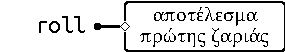
\includegraphics[scale=\scaling]{illustrations/roll-1.pdf}
\captionof{figure}{\label{image:roll-init}Αρχικά, η τιμή της μεταβλητής \pyinline{roll} αντιστοιχεί στο αποτέλεσμα της πρώτης ζαριάς.}}
\marginnote[-8pt]{\center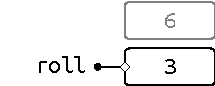
\includegraphics[scale=\scaling]{illustrations/roll-2.pdf}
\captionof{figure}{\label{image:roll-again}Στη συνέχεια, η \pyinline{roll} χρησιμοποιείται για το αποτέλεσμα της δεύτερης ζαριάς και η τιμή της τροποποιείται. Το αποτέλεσμα της πρώτης ζαριάς δεν είναι πια διαθέσιμο.}}
Κάποια στιγμή θα πρέπει να ελεγχθεί αν η δεύτερη ζαριά του παίκτη είναι ίση με την πρώτη, για να διαπιστωθεί αν κέρδισε ή όχι. Το πρόβλημα είναι ότι, με το πρόγραμμα ως έχει, αυτό είναι αδύνατο: Όταν ρίχνεται η δεύτερη ζαριά, το αποτέλεσμά της ονομάζεται και πάλι \pyinline{roll}. Η προηγούμενη τιμή της \pyinline{roll}, η τιμή της πρώτης ζαριάς, δεν είναι πια διαθέσιμη και δεν μπορεί να γίνει σύγκριση μεταξύ των δύο τιμών (δείτε σχετικά και τα σχήματα~\ref{image:roll-init} και~\ref{image:roll-again}).

\clearpage
\marginnote{\center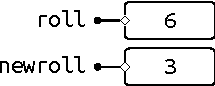
\includegraphics[scale=\scaling]{illustrations/roll-3.pdf}
\captionof{figure}{Το αποτέλεσμα της δεύτερης ζαριάς ονομάζεται \pyinline{newroll}. Οι δυο ζαριές, οι τιμές \pyinline{roll} και \pyinline{newroll} μπορούν να συγκριθούν μεταξύ τους.}}%
\vspace{-3\parskip}%
Για να λυθεί το πρόβλημα θα χρησιμοποιήσουμε μια \emph{διαφορετική μεταβλητή}, ένα διαφορετικό όνομα για τη δεύτερη ζαριά.

% src/craps.2.py: ο παίκτης ξαναρίχνει (στη newroll)
\pysrc[firstline=18,lastline=27]{src/craps.2.py}{plain}{continued}
\pysrc[firstline=28,lastline=29]{src/craps.2.py}{}{}

Τώρα μπορούμε να συγκρίνουμε τη δεύτερη ζαριά με την πρώτη, δηλαδή την τιμή της \pyinline{newroll} με εκείνη της \pyinline{roll} για να εξετάσουμε αν ο παίκτης κέρδισε ή όχι.

% src/craps.2.py: έλεγχος αποτελέσματος, χωρίς break (δεύτερη ζαριά)
\pysrc[firstline=28,lastline=29]{src/craps.2.py}{plain}{continued}
\pysrc[firstline=30,lastline=34]{src/craps.2.py}{}{craps}

%%%%%%%%

\section{Ξανά Και Ξανά}

\begin{question}
Η τρίτη περίπτωση ακόμα δεν είναι ολοκληρωμένη. Αν ο παίκτης δεν κερδίσει, ούτε χάσει με την πρώτη, ίσως χρειαστεί να ρίξει περισσότερες από μία επιπλέον ζαριές. Πώς θα κάνουμε τις υπάρχουσες εντολές για τη δεύτερη ζαριά να επαναλαμβάνονται; 
\end{question}

Κάθε γλώσσα προγραμματισμού προσφέρει \emph{επαναληπτικές δομές}, %
\marginnote[-58pt]{Στην Python, η βασική επαναληπτική δομή είναι η \pyinline{while}, η οποία μπορεί να χρησιμοποιηθεί σε κάθε περίπτωση, ενώ για συγκεκριμένου είδους επαναλήψεις υπάρχει και η δομή \pyinline{for}.}%
\marginnote{Η επαναληπτική δομή \pyinline{while} συνοδεύεται από μια \emph{συνθήκη συνέχειας}. Η συνθήκη ελέγχεται στην αρχή κάθε νέου κύκλου της επανάληψης και μπορεί να είναι αληθής (\pyinline{True}) ή ψευδής (\pyinline{False}). Όσο η συνθήκη είναι αληθής, η επανάληψη συνεχίζεται για άλλον έναν κύκλο.}
%\marginnote{Μην παραλείπετε το σύμβολο \pyinline{:} μετά την συνθήκη.}%
\marginnote{%
\center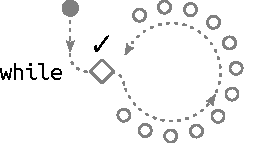
\includegraphics[scale=\scaling]{illustrations/iteration-true.pdf}
\captionof{figure}{Η τετριμμένη συνθήκη \pyinline{True} που ελέγχεται εδώ από τη \pyinline{while} είναι πάντα αληθής, κι έτσι η συγκεκριμένη επανάληψη θα ξεκινήσει σίγουρα και δεν πρόκειται να διακοπεί λόγω της συνθήκης.}%
}
δηλαδή τρόπους να εκφράσει κανείς ότι ένα σύνολο εντολών θα πρέπει να επαναλαμβάνεται.%

Μια τέτοια επαναληπτική δομή θα χρειαστεί να προσθέσουμε στην τρίτη περίπτωση, όπου ο παίκτης ούτε κερδίζει, ούτε χάνει με την πρώτη. \emph{Μέσα} στην επανάληψη θα τοποθετήσουμε τις εντολές που υλοποιούν την ρίψη των ζαριών και ελέγχουν το αποτέλεσμα. Οι εντολές γράφονται μόνο μια φορά αλλά εκτελούνται ξανά και ξανά.

% src/craps.3: επανάληψη ρίψεων 
\pysrc[firstline=18,lastline=20]{src/craps.3.py}{plain}{continued}
\pysrc[firstline=21,lastline=22]{src/craps.3.py}{}{}
\clearpage
\marginnote{Οι εντολές που ακολουθούν τη \pyinline{while} είναι στοιχισμένες δεξιότερα. Η στοίχιση αυτή επιτυγχάνεται εισάγοντας κενά πριν από τις εντολές, τα οποία υποδηλώνουν ότι αυτές οι εντολές ``ανήκουν'' στη \pyinline{while} και θα επαναλαμβάνονται. Η πρώτη εντολή μετά τη \pyinline{while} που δεν θα είναι στοιχισμένη δεξιότερα δεν θα επαναλαμβάνεται, αλλά θα εκτελεστεί μόνο μια φορά, όταν η επανάληψη τερματιστεί.}%
\vspace{-3\parskip}%
\pysrc[firstline=23,lastline=31]{src/craps.3.py}{plain}{}

%%%%%%%%

\section{Είναι Σημαντικό Να Έχεις Στόχους}

\begin{question}
Οι επαναλαμβανόμενες ρίψεις των ζαριών πρέπει κάποτε να σταματούν. Πώς τερματίζω την επαναληπτική διαδικασία;
\end{question}

% Οι εντολές που εμφωλεύτηκαν στην επαναληπτική δομή εκτελούνται \emph{συνεχώς} και ο παίκτης καλείται να ρίχνει ζαριές ακόμα κι όταν το παιχνίδι (θα πρέπει να) τελειώσει. 
Ήδη το πρόγραμμά μας ελέγχει μετά από κάθε ζαριά την έκβασή της. Υπάρχουν κι εδώ τρεις πιθανές περιπτώσεις: νίκη (ο παίκτης φέρνει ζαριά ίση με τον στόχο), ήττα (ο παίκτης φέρνει \pyinline{7}) και συνέχεια της επανάληψης (σε οποιαδήποτε άλλη περίπτωση). Στις δύο πρώτες περιπτώσεις η επανάληψη θα πρέπει να τερματιστεί. Ένας απλός τρόπος για να επιτευχθεί αυτό είναι με την προσθήκη της εντολής \pyinline{break}, η οποία διακόπτει άμεσα τον κύκλο της επανάληψης.

% src/craps.3: έλεγχος αποτελέσματος με break (δεύτερη ζαριά)
\marginnote[-78pt]{%
\center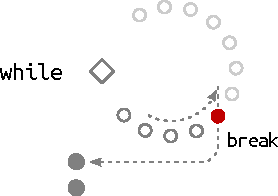
\includegraphics[scale=\scaling]{illustrations/iteration-break.pdf}%
\captionof{figure}{Η \pyinline{break} διακόπτει και τερματίζει \emph{άμεσα} τον κύκλο της επανάληψης, χωρίς να ελεγχθεί η συνθήκη συνέχειας. Οι εντολές μετά την \pyinline{break} αγνοούνται και η εκτέλεση συνεχίζεται από την πρώτη εντολή που ακολουθεί την επανάληψη.}%
}
\marginnote{Για να κατανοήσετε καλύτερα τι σημαίνει η άμεση διακοπή της επανάληψης όταν εκτελεστεί η \pyinline{break}, δοκιμάστε να τοποθετήσετε τις \pyinline{print} \emph{μετά} τις \pyinline{break}. Θα διαπιστώσετε ότι τα μηνύματα δεν θα εμφανιστούν ποτέ.} 
\marginnote{Η \pyinline{else} δεν είναι υποχρεωτική σε μια δομή επιλογής και παραλείπεται όταν δεν υπάρχουν εντολές να εκτελεστούν στην τελευταία περίπτωση.} 
\pysrc[firstline=32,lastline=34]{src/craps.3.py}{plain}{continued}
\pysrc[firstline=35,lastline=36]{src/craps.3.py}{}{continued}
\pysrc[firstline=37,lastline=38]{src/craps.3.py}{plain}{continued}
\pysrc[firstline=39,lastline=40]{src/craps.3.py}{}{craps}

Η χρήση της \pyinline{break} είναι μια πρακτική που δεν ακολουθείται από όλους. Ορισμένοι θεωρούν ότι ο κώδικας είναι πιο κατανοητός όταν υπάρχει ένα μοναδικό σημείο εξόδου από την επανάληψη: η συνθήκη συνέχειας. Θα εξετάσουμε μια εκδοχή στην οποία ο κύκλος της επανάληψης δεν διακόπτεται άμεσα με την \pyinline{break} αλλά μόνο όταν η συνθήκη συνέχειας ελεγχθεί και διαπιστωθεί ότι είναι ψευδής.

% Είναι σημαντικό να συγκρίνετε το νέο αυτό πρόγραμμα με το προηγούμενο και να κατανοήσετε τον μηχανισμό τερματισμού της επανάληψης σε κάθε περίπτωση.

Θα χρησιμοποιήσουμε μια \emph{λογική} %
\marginnote[2pt]{Υπάρχουν μόνο δύο \emph{λογικές} τιμές: \pyinline{True} ή \pyinline{False}.}%, οι οποίες είναι τύπου \pyinline{bool}.}%
μεταβλητή \pyinline{over} για να ``θυμάται'' το πρόγραμμά μας αν το παιχνίδι έχει τελειώσει. Αρχικά, πριν την επανάληψη, η \pyinline{over} ορίζεται ως ψευδής (\pyinline{False}).

% src/craps.4: αρχική τιμή για την over
\pysrc[firstline=18,lastline=20]{src/craps.4.py}{plain}{continued}
\pysrc[firstline=21,lastline=22]{src/craps.4.py}{}{}

\clearpage
Στην αρχή κάθε κύκλου της επανάληψης, ελέγχεται η συνθήκη συνέχειας \pyinline{not over}\marginnote[2pt]{Το \pyinline{not} χρησιμοποιείται πριν από μια συνθήκη και \emph{αντιστρέφει} την τιμή της: όταν μια συνθήκη είναι ψευδής τότε η αντίστροφή της είναι αληθής και το ανάποδο.} κι ένας νέος κύκλος ξεκινά μόνο εφόσον η \pyinline{over} εξακολουθεί να είναι ψευδής.

% src/craps.4: επαναληπτικές ρίψεις (με την over)
\pysrc[firstline=21,lastline=22]{src/craps.4.py}{plain}{continued}
\pysrc[firstline=23,lastline=24]{src/craps.4.py}{}{}

Η συνθήκη συνέχειας της επανάληψης θα μπορούσε εναλλακτικά να γραφτεί και με τους δύο ακόλουθους τρόπους:

\begin{pycode}
    # επανάληψη ρίψεων
    while over == False
\end{pycode}

\marginnote[28pt]{Με το \pyinline{!=} ελέγχεται αν δύο τιμές είναι διαφορετικές.}%
\begin{pycode}
    # επανάληψη ρίψεων
    while over != True
\end{pycode}

Η τιμή της \pyinline{over} θα πρέπει να αλλάζει σε αληθής (\pyinline{True}) όταν ο παίκτης κερδίσει ή χάσει -- εκεί δηλαδή όπου στην προηγούμενη εκδοχή συναντούσαμε την \pyinline{break}. 

\marginnote[18pt]{%
\center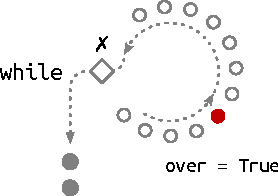
\includegraphics[scale=\scaling]{illustrations/iteration-boolean.pdf}
\captionof{figure}{Όταν η \pyinline{over} πάρει τιμή \pyinline{True}, η επανάληψη \emph{δεν} θα διακοπεί άμεσα, γιατί η συνθήκη \pyinline{not over} της \pyinline{while} δεν ελέγχεται συνεχώς. Η επανάληψη θα διακοπεί όταν ελεγχθεί η συνθήκη της \pyinline{while}, δηλαδή αφού τελειώσει ο κύκλος της επανάληψης.}%
}
% [suggested] Θα μπορούσαμε να προσθέσουμε κι εδώ ένα σχόλιο ότι αν οι print τοποθετηθούν *μετά* τις over = False, θα εκτελεστούν ούτως ή άλλως.
% src/craps.4: έλεγχος αποτελέσματος (με την over)
\pysrc[firstline=34,lastline=37]{src/craps.4.py}{plain}{continued}
\pysrc[firstline=38,lastline=38]{src/craps.4.py}{}{continued}
\pysrc[firstline=39,lastline=41]{src/craps.4.py}{plain}{continued}
\pysrc[firstline=42,lastline=42]{src/craps.4.py}{}{craps}

Στην εκδοχή αυτή η επανάληψη \emph{δεν} θα σταματήσει άμεσα όταν η \pyinline{over} γίνει αληθής, αλλά όταν ελεγχθεί η συνθήκη συνέχειας και διαπιστωθεί ότι η \pyinline{over} είναι αληθής.

Μεταβλητές όπως η \pyinline{over} που παίρνουν μόνο δύο τιμές και χρησιμοποιούνται ως ένδειξη ότι κάποιο γεγονός έχει συμβεί ή όχι ονομάζονται συχνά \emph{σημαίες} (flags).

%%%%%%%%

\section{Κάν'το Μου Λιανά}

\begin{question}
Το πρόγραμμα λειτουργεί, αλλά δεν μου αρέσει ο τρόπος που είναι γραμμένο. Οι εντολές για την ρίψη μιας ζαριάς επαναλαμβάνονται αυτούσιες σε δύο σημεία του προγράμματος. 
\end{question}

Οι ίδιες εντολές που προσομοιώνουν τη ρίψη των ζαριών χρησιμοποιούνται τόσο στην αρχική ζαριά όσο και στις επαναλαμβανόμενες ζαριές. 
Αυτές οι εντολές δεν είναι ούτε αναγκαίο, ούτε σκόπιμο να ξαναγράφονται. Ουσιαστικά, αποτελούν ένα ενιαίο σύνολο και υλοποιούν μια συγκεκριμένη λειτουργία. Μπορούμε λοιπόν να τις τοποθετήσουμε μέσα σ' ένα \emph{υποπρόγραμμα}, %
\marginnote[-112pt]{Tα υποπρογράμματα στην Python και σε πολλές άλλες γλώσσες έχουν τη μορφή \emph{συναρτήσεων}. Έχουν ένα όνομα και μια (προαιρετική) σειρά \emph{παραμέτρων}, εντός παρενθέσεων. Όταν κληθούν, οι συναρτήσεις δέχονται τιμές για τις παραμέτρους, τις \emph{επεξεργάζονται} και \emph{επιστρέφουν} ένα αποτέλεσμα.}
\marginnote[-18pt]{Έχουμε ήδη χρησιμοποιήσει συναρτήσεις που παρέχει έτοιμες η Python, όπως η \pyinline{print()} και η \pyinline{input()}, αλλά και συναρτήσεις που ανήκουν σε βιβλιοθήκες, όπως \pyinline{time.sleep()} και η \pyinline{random.randint()}. Τα προγράμματά μας καλούν αυτές τις συναρτήσεις κι αυτές εκτελούνται, παρέχοντας συγκεκριμένες λειτουργίες.}%
δημιουργώντας ένα κλειστό ``εξάρτημα'' που υλοποιεί τη λειτουργία της ρίψης των ζαριών.% και η οποία έχει ως αποτέλεσμα το άθροισμα των ενδείξεων των δύο ζαριών.

\clearpage
\marginnote{\center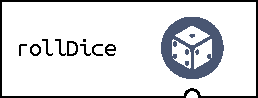
\includegraphics[scale=\scaling]{illustrations/rollDice.pdf}
\captionof{figure}{Η συνάρτηση \pyinline{rollDice} είναι ένα ανεξάρτητο τμήμα κώδικα, ένα αυτόνομο ``εξάρτημα'' που επιτελεί μια συγκεκριμένη λειτουργία. Όταν κληθεί, η συνάρτηση προσομοιώνει τη ρίψη δύο ζαριών κι επιστρέφει το άθροισμα των ενδείξεών τους.}}%
\vspace{-3\parskip}%
Το υποπρόγραμμα \pyinline{rollDice()} που ακολουθεί δεν δέχεται \emph{παραμέτρους} (γιατί δεν χρειάζεται εξωτερικές τιμές για να λειτουργήσει), και \emph{επιστρέφει} το άθροισμα των ενδείξεων των δύο ζαριών.

% src/craps.5.py: το υποπρόγραμμα rollDice()
\marginnote[10pt]{Ο ορισμός μιας συνάρτησης ξεκινά με τη λέξη \pyinline{def} και ακολουθείται από το όνομα της συνάρτησης και τις παραμέτρους της, μέσα σε παρενθέσεις.}%
%\marginnote{Μην παραλείπετε το σύμβολο \pyinline{:} στο τέλος της πρώτης γραμμής.}%
\marginnote{Οι εντολές μετά την πρώτη γραμμή είναι στοιχισμένες δεξιότερα. Η στοίχιση αυτή υποδηλώνει ότι οι εντολές αυτές ``ανήκουν'' στη συνάρτηση και θα εκτελεστούν όταν αυτή \emph{κληθεί}.}%
\marginnote{Το αποτέλεσμα της συνάρτησης (όταν υπάρχει) \emph{επιστρέφεται} με την \pyinline{return}.}%
\marginnote{Το ειδικό σχόλιο στην αρχή της συνάρτησης, ανάμεσα στα 3 διπλά εισαγωγικά, χρησιμοποιείται για να περιγράψει τη λειτουργία της. Είναι προαιρετικό, όπως όλα τα σχόλια.}%
\pysrc[firstline=2,lastline=15]{src/craps.5.py}{}{}

Σημειώστε ότι οι μεταβλητές \pyinline{dice1}, \pyinline{dice2} και \pyinline{roll} είναι \emph{τοπικές} στο υποπρόγραμμα. Δημιουργούνται κάθε φορά που αυτό καλείται και παύουν να υπάρχουν όταν ολοκληρωθεί η εκτέλεσή του. Η μεταβλητή \pyinline{roll} του κύριου προγράμματος είναι διαφορετική από εκείνη του υποπρογράμματος.

\marginnote[18pt]{\center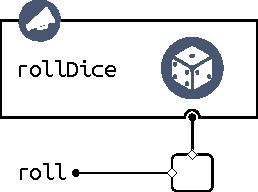
\includegraphics[scale=\scaling]{illustrations/rollDice-call.pdf}
\captionof{figure}{Όταν κληθεί η \pyinline{rollDice()} εκτελούνται οι εντολές της και η συνάρτηση επιστρέφει μια τιμή. Για την αρχική ζαριά, η τιμή αυτή αποδίδεται στη μεταβλητή \pyinline{roll} του κύριου προγράμματος.}}%

Προς το παρόν έχουμε μόνο \emph{ορίσει} το υποπρόγραμμα. Για να το χρησιμοποιήσουμε, ενεργοποιώντας την εκτέλεση των εντολών του, πρέπει να το \emph{καλέσουμε} στα δύο σημεία του προγράμματος όπου ο χρήστης ρίχνει τα ζάρια, \emph{αντικαθιστώντας} τις υπάρχουσες εντολές.

Έτσι, στο σημείο όπου ρίχνεται η αρχική ζαριά, τώρα καλούμε τη \pyinline{rollDice()}, ονομάζοντας \pyinline{roll} το αποτέλεσμα που επιστρέφεται.

% src/craps.5.py: κλήση υποπρογράμματος για την αρχική ζαριά
\pysrc[firstline=16,lastline=17]{src/craps.5.py}{}{continued}
\pysrc[firstline=18,lastline=19]{src/craps.5.py}{plain}{}

Παρομοίως, στο σημείο όπου ρίχνεται η επαναλαμβανόμενη ζαριά, καλούμε και πάλι τη \pyinline{rollDice()}, ονομάζοντας \pyinline{newroll} το αποτέλεσμα που επιστρέφεται.

% src/craps.5.py: κλήση υποπρογράμματος για την επαναλαμβανόμενη ζαριά
\pysrc[firstline=30,lastline=31]{src/craps.5.py}{plain}{continued}
\pysrc[firstline=32,lastline=33]{src/craps.5.py}{}{continued}
\pysrc[firstline=34,lastline=35]{src/craps.5.py}{plain}{craps}

% [suggested] Μικρός σχολιασμός

%%%%%%%%

\section{Πλήρες Πρόγραμμα}

\pysrc{src/craps.final.py}{}{craps}

%%%%%%%%

\section{Ασκήσεις}

\begin{exercise}
Ο Ευκλείδης, στο έβδομο βιβλίο των \emph{Στοιχείων} του, περιγράφει μια μέθοδο για την εύρεση του μέγιστου κοινού διαιρέτη δύο ακεραίων. Τα Στοιχεία γράφτηκαν περίπου το 300 π.Χ. και η μέθοδος καθεαυτή θεωρείται ακόμα παλιότερη, γι' αυτό και ο Donald Knuth, στο εμβληματικό βιβλίο του \emph{The Art of Computer Programming}, τη χαρακτηρίζει ως τον ``παππού'' όλων των αλγορίθμων, γιατί είναι ο παλαιότερος γνωστός αλγόριθμος που χρησιμοποιείται ακόμα και σήμερα.

Μπορεί κανείς να βρει πολλές διαφορετικές εκδοχές του αλγορίθμου, αλλά βασικά ο αλγόριθμος μπορεί να συνοψιστεί ως εξής:
\begin{quote}
Αφαίρεσε τον μικρότερο αριθμό από τον μεγαλύτερο και επανάλαβε τη διαδικασία μέχρι οι δύο αριθμοί να γίνουν ίσοι. Η τιμή των δύο αριθμών όταν τελειώσει η διαδικασία είναι ο μέγιστος κοινός διαιρέτης τους.
\end{quote}
Γράψτε ένα πρόγραμμα το οποίο ζητάει από το χρήστη δύο ακέραιους αριθμούς και υπολογίζει τον μέγιστο κοινό διαιρέτη τους, χρησιμοποιώντας τη μέθοδο του Ευκλείδη.
% [suggested] Χρειάζεται κάποια υπόδειξη; Π.χ. για το a = a - b;
\solutionlink{craps}{eukleides.py}
\end{exercise}

\begin{exercise} % Collatz
Το 1937, ο γερμανός μαθηματικός Lothar Collatz διατύπωσε τον παρακάτω ισχυρισμό, ο οποίος παραμένει αναπόδεικτος:
\begin{quote}
Επιλέξτε έναν θετικό ακέραιο n. Αν είναι άρτιος διαιρέστε τον με το 2, ενώ αν είναι περιττός πολλαπλασιάστε τον με το 3 και προσθέστε μια μονάδα. Επαναλάβετε τη διαδικασία με τον νέο αριθμό που θα προκύψει. Από οποιονδήποτε αριθμό n κι αν ξεκινήσετε, θα καταλήξετε στον αριθμό 1.
\end{quote}
Η εικασία %
\marginnote{\upshape\href{http://xkcd.com/710/}{\url{xkcd.com/710/}}}
έχει επαληθευτεί αριθμητικά μέχρι και για αριθμούς της τάξης των 6 δισεκατομμυρίων δισεκατομμυρίων, ωστόσο δεν υπάρχει αναλυτική μαθηματική απόδειξη. Θεωρητικά υπάρχει πάντα το ενδεχόμενο ένας ακόμα μεγαλύτερος αριθμός να παραβιάζει την εικασία!

Γράψτε ένα πρόγραμμα %
\marginnote{Για να διαπιστώσετε αν ένας αριθμός είναι περιττός ελέγξτε αν το υπόλοιπο της διαίρεσής του με το 2 είναι το 1.}%
το οποίο θα διαβάζει από το χρήστη τον αριθμό εκκίνησης n, θα επαναλαμβάνει τη διαδικασία 
που περιγράφεται παραπάνω και θα εμφανίζει τους διαδοχικούς αριθμούς που προκύπτουν από αυτή, έως ότου η διαδικασία καταλήξει στον αριθμό 1. Μπορείτε να εμπλουτίσετε το πρόγραμμά σας, ώστε μετά το τέλος της διαδικασίας να εμφανίζει το χρόνο τερματισμού, δηλαδή το συνολικό αριθμό των βημάτων που απαιτήθηκαν, αλλά και το σημείο πλημμυρίδας, δηλαδή τον μεγαλύτερο αριθμό που προέκυψε κατά την εκτέλεση της διαδικασίας.

\begin{note}
Για παράδειγμα, ξεκινώντας από το n=6 δημιουργείται η παρακάτω ακολουθία, με χρόνο τερματισμού τα 8 βήματα και σημείο πλημμυρίδας το 16:
\begin{center}
6\quad 3\quad 10\quad 5\quad 16\quad 8\quad 4\quad 2\quad 1
\end{center}
\end{note}
\mbox{}\vspace{-24pt}\solutionlink{craps}{collatz.py}
\end{exercise}

\begin{exercise}
Γράψτε μια συνάρτηση \pyinline{flip()}, η οποία θα μιμείται τη ρίψη ενός νομίσματος, επιστρέφοντας με τυχαίο τρόπο είτε το \pyinline{0}, είτε το \pyinline{1}.

Κατασκευάστε πρόγραμμα το οποίο θα παίζει \emph{Κορώνα-Γράμματα} με το χρήστη. Το πρόγραμμα θα ρωτάει τον παίκτη αν επιλέγει Κορώνα ή Γράμματα (\pyinline{0} για Κορώνα και \pyinline{1} για Γράμματα), θα προσομοιώνει τη ρίψη του νομίσματος καλώντας τη \pyinline{flip} και θα ενημερώνει τον παίκτη αν κέρδισε ή έχασε. Κάντε το πρόγραμμά σας επαναληπτικό, με το παιχνίδι να σταματά όταν ο χρήστης σε κάποιο γύρο δεν επιλέξει ούτε Κορώνα, ούτε Γράμματα.
\solutionlink{craps}{headstails.py}

Μπορείτε να τροποποιήσετε το πρόγραμμά σας έτσι ώστε να ``κλέβει'' το χρήστη. Χωρίς να γίνεται ρίψη του νομίσματος, κάντε το πρόγραμμα ν' ανακοινώνει ότι το αποτέλεσμα της ρίψης του κέρματος ήταν το αντίθετο από αυτό που επέλεξε ο παίκτης.
\solutionlink{craps}{headstails-cheat.py}

% [modified] 
Για να γίνει το πρόγραμμα πιο πειστικό, καλό θα ήταν να μην κερδίζει πάντα, αλλά ν' αφήνει μερικές φορές και το χρήστη να κερδίσει και να αισθανθεί τυχερός... Σε αυτές τις περιπτώσεις, χωρίς να γίνεται ρίψη του νομίσματος, το πρόγραμμα θ' ανακοινώνει ότι το αποτέλεσμα της ρίψης του κέρματος ήταν το ίδιο με αυτό που επέλεξε ο παίκτης.
\solutionlink{craps}{headstails-cheat-probability.py}

\begin{note}
Υπόδειξη: Πριν την ανακοίνωση του ``στημένου'' αποτελέσματος, το πρόγραμμα μπορεί να επιλέγει τυχαία έναν αριθμό από το \pyinline{1} μέχρι το \pyinline{100}. Αν αυτός ο αριθμός ξεπερνά ένα υψηλό ``κατώφλι'', τότε το πρόγραμμα θ' ανακοινώνει στον παίκτη ότι κέρδισε. 

\begin{pynew}
win = random.randint(1,100)
if win > 90:
    # ο παίκτης κερδίζει
    |...|
else:
    # ο παίκτης χάνει
    |...|
\end{pynew}
\end{note}

%\begin{note}
%Αν δυσκολευτείτε, μελετήστε τον τρόπο με τον οποίο η \pyinline{rollDice} κάνει κάτι ανάλογο με τις έξι πιθανά αποτελέσματα της ρίψης ενός ζαριού.
%\end{note}

%Πρώτα βεβαιωθείτε ότι το νόμισμα που κατασκευάσατε είναι δίκαιο. Κατασκευάστε ένα πρόγραμμα που καλεί επαναληπτικά την συνάρτηση (για παράδειγμα ένα εκατομμύριο φορές) % δεν ξέρουν να το κάνουν αυτό % και μετράει ποιο ποσοστό των ρίψεων είχε ως αποτέλεσμα το \pyinline{0}.
% πιθανώς θα μπορούσαμε να τους δώσουμε έτοιμο τον κώδικα για να το κάνουν αυτό (ή ένα τμήμα του).
%Αν θεωρείτε ότι η συνάρτηση \pyinline{flip} παράγει δίκαια αποτελέσματα, τότε αναπτύξτε ένα πρόγραμμα το οποίο θα παίζει επαναληπτικά με το χρήστη το παιχνίδι Κορώνα - Γράμματα.
\end{exercise}

\begin{exercise}
Να κατασκευάσετε ένα πρόγραμμα το οποίο θα παίζει επαναληπτικά το γνωστό παιχνίδι «Πέτρα-Ψαλίδι-Χαρτί» με το χρήστη. Σε κάθε γύρο, το πρόγραμμα θα ζητά από το χρήστη την επιλογή του (\pyinline{1} για την Πέτρα, \pyinline{2} για το Ψαλίδι ή \pyinline{3} για το Χαρτί) και στη συνέχεια θα εμφανίζει τη δική του επιλογή και θα ανακοινώνει το νικητή του γύρου. Αν ο χρήστης πληκτρολογήσει οτιδήποτε εκτός από τις τρεις έγκυρες επιλογές τότε θεωρείται ότι επιθυμεί να τερματίσει το παιχνίδι. 
\solutionlink{craps}{rps.py}

Μπορείτε να δοκιμάσετε και παραλλαγές του παιχνιδιού: τροποποιήστε το πρόγραμμα έτσι ώστε να επιλέγει από τις διαφορετικές κινήσεις με διαφορετική πιθανότητα ή κάντε το πρόγραμμα να κλέβει (μερικές φορές), επιλέγοντας κίνηση με βάση την κίνηση του χρήστη.
\solutionlink{craps}{rps-cheat.py}
\end{exercise}

\begin{exercise}
Το «Ανάμεσα» ή «Acey Ducey» είναι ένα παιχνίδι με χαρτιά. Ο ένας παίκτης (η «μάνα») τραβάει δύο χαρτιά από την τράπουλα και τα δείχνει στο δεύτερο παίκτη. Εκείνος με την σειρά του στοιχηματίζει ένα ποσό και νικάει όταν το τρίτο χαρτί είναι ανάμεσα στα δύο πρώτα. Όσο πιο απίθανο είναι να νικήσει ένας παίκτης, τόσο μεγαλύτερο είναι το ποσό που θα κερδίσει. Συγκεκριμένα, αν υπάρχουν d χαρτιά ανάμεσα στα δύο πρώτα, τότε το ποσό που κερδίζει ο παίκτης σε περίπτωση νίκης θα είναι 12/d φορές το ποσό που στοιχημάτισε.

\begin{note}
Για παράδειγμα, αν τα δύο πρώτα χαρτιά είναι το 5 και το 8, τότε ο δεύτερος παίκτης θα νικήσει αν το επόμενο χαρτί είναι το 6 ή το 7 (d=2). Στην περίπτωση αυτή θα κερδίσει 6 φορές το ποσό που στοιχημάτισε.
\end{note}

Θεωρήστε ότι τα χαρτιά που χρησιμοποιούνται είναι από το 1 μέχρι και το 13 (τα τρία τελευταία αντιστοιχούν στον βαλέ, τη ντάμα και τον ρήγα). Αναπτύξτε πρόγραμμα το οποίο παράγει τυχαία τα δύο πρώτα χαρτιά της μάνας. Αυτά θα πρέπει να διαφέρουν αριθμητικά τουλάχιστον κατά δύο μονάδες, ώστε να υπάρχει περιθώριο για τουλάχιστον ένα χαρτί ανάμεσά τους (d\,$\geq$1), αλλιώς η μάνα θα πρέπει να μοιράσει δύο νέα χαρτιά. Στη συνέχεια, το πρόγραμμα ρωτά τον παίκτη το ποσό που επιθυμεί να στοιχηματίσει και παράγει το τρίτο χαρτί, εμφανίζοντας κατάλληλο μήνυμα με το ποσό που κέρδισε ή έχασε ο δεύτερος παίκτης.
\solutionlink{craps}{aceyducey.py}
\end{exercise}

%%%%%%%%

\section*{}
\vspace{-6\parskip}
\hrulefill

%\begin{theory}{Τελεστές και Εκφράσεις}
%\end{theory}

%\begin{theory}{Δομή Πολλαπλής Επιλογής}
%Πρόκειται για μια δομή \emph{πολλαπλής επιλογής}, αφού χρειάζεται να διακρίνουμε ανάμεσα σε περισσότερες από δύο περιπτώσεις.
%\end{theory}

\begin{theory}{Δομή Επανάληψης}
Η δομή επανάληψης μας δίνει τη δυνατότητα να περιγράφουμε διαδικασίες που επαναλαμβάνονται. Ίσως αρχικά αυτό να μην ακούγεται ιδιαίτερα εντυπωσιακό, γρήγορα όμως ανακαλύπτουμε ότι οι περισσότερες υπολογιστικές διαδικασίες είναι εγγενώς επαναληπτικές (αυτό περιλαμβάνει και τα περισσότερα \emph{παιχνίδια}) και είναι απαραίτητος ένας συμπαγής τρόπος περιγραφής τους. Με τη δομή επανάληψης περιγράφουμε τα βήματα ενός μόνο κύκλου, ακόμα κι αν τελικά αυτά τα βήματα θα εκτελεστούν πάρα πολλές φορές. 'Η ακόμα κι αν δεν γνωρίζουμε εκ των προτέρων πόσες φορές θα εκτελεστούν. Από μία άποψη, στις υπολογιστικές μας συσκευές ταιριάζει πολύ η δομή επανάληψης: σε αντίθεση με τους ανθρώπους, έχουν τη δυνατότητα να εκτελούν αδιαμαρτύρητα τα ίδια βήματα, ξανά και ξανά.
\end{theory}

\begin{theory}{Αναγνωσιμότητα και Break}
Σε μια επανάληψη μπορούμε να χρησιμοποιήσουμε μία ή και περισσότερες \pyinline{break}. Κάθε \pyinline{break} ανοίγει μια πόρτα εξόδου από τον κύκλο της επανάληψης. Επομένως, για να γνωρίζει κανείς πότε θα τερματιστεί μια επανάληψη θα πρέπει να αναζητήσει τις \pyinline{break} μέσα στην επανάληψη και να διαπιστώσει υπό ποιες συνθήκες θα εκτελεστούν. Αντίθετα, χωρίς την \pyinline{break}, η έξοδος από την επανάληψη γίνεται από ένα και μοναδικό σημείο: την συνθήκη συνέχειας. Η επανάληψη τερματίζεται μόνο όταν η συνθήκη συνέχειας ελεγχθεί και διαπιστωθεί ότι είναι ψευδής. Αρκεί λοιπόν να κοιτάξει κανείς την συνθήκη συνέχειας για να γνωρίζει πότε θα τερματιστεί μια επανάληψη. Φαίνεται λοιπόν ότι η άμεση διακοπή μιας επανάληψης με την \pyinline{break} είναι μεν συχνά βολική, όμως χωρίς την \pyinline{break} προκύπτουν προγράμματα που είναι περισσότερο κατανοητά και ευανάγνωστα. Αυτό είναι εξαιρετικά σημαντικό για κάποιους και πολύ λιγότερο για άλλους...
\end{theory}

\begin{theory}{Υποπρογράμματα}
Το μεγαλύτερο πλεονέκτημα που προκύπτει από τη χρήση υποπρογραμμάτων (και γίνεται πολύ εμφανέστερο καθώς τα προβλήματα και τα αντίστοιχα προγράμματα μεγαλώνουν) είναι ότι είμαστε ``αναγκασμένοι'' να αναλύουμε τα προβλήματα και να τ' αντιμετωπίζουμε \emph{τμηματικά}. Κάθε φορά εστιάζουμε την προσοχή μας σε μικρότερα κι απλούστερα κομμάτια του γενικού προβλήματος και στη συνέχεια, συνθέτουμε τη λύση, συναρμολογώντας τα κομμάτια αυτά. Στα κεφάλαια που ακολουθούν θα χρησιμοποιήσουμε περισσότερο τα υποπρογράμματα και θα αναφερθούμε εκτενέστερα στα πλεονεκτήματα που πηγάζουν από τη χρήση τους.
\end{theory}

\begin{theory}{Τυχαίοι Αριθμοί}
Η παραγωγή τυχαίων αριθμών έχει πολλές και σημαντικές εφαρμογές, όπως στην στατιστική, τις προσομοιώσεις και τα παιχνίδια, όμως η σημαντικότερη εφαρμογή της είναι στην \emph{κρυπτογραφία}. Υπάρχουν αρκετές υπολογιστικές μέθοδοι για να παράγει κανείς τυχαίους αριθμούς. Όλες τους ονομάζονται και \emph{γεννήτριες ψευδο-τυχαίων αριθμών} γιατί η αλήθεια είναι ότι οι αριθμοί που παράγουν \emph{φαίνονται} τυχαίοι, αλλά δεν είναι. Υπάρχουν μάλιστα και ειδικά στατιστικά κριτήρια που μετρούν πόσο απρόβλεπτες είναι οι ακολουθίες αριθμών που παράγονται. Η Python (και άλλες γλώσσες) χρησιμοποιoύν έναν αλγόριθμο που ονομάζεται Mersenne-Twister, ο οποίος είναι επαρκής για τις συνήθεις χρήσεις αλλά όχι για την κρυπτογραφία.
\end{theory}

\begin{theory}{Ζάρια, Χαρτιά και Τυχερά Παιχνίδια}
Πολλά από τα παραδείγματα με τα οποία θ' ασχοληθούμε είναι παιχνίδια με ζάρια ή χαρτιά. Τα επιλέξαμε επειδή θεωρούμε ότι είναι διασκεδαστικά και έχουν αλγοριθμικό ενδιαφέρον. Ωστόσο, ο \emph{εθισμός} σε αυτά τα παιχνίδια αποτελεί σημαντικότατο πρόβλημα. Τα \emph{ηλεκτρονικά} τυχερά παιχνίδια έχουν κι άλλες υπόγειες διαστάσεις. Μέσα από ορισμένες ασκήσεις, ελπίζουμε να κατανοήσετε πως όταν παίζεις ένα τυχερό παιχνίδι μ' ένα πρόγραμμα, ίσως το παιχνίδι να μην αφήνει και τόσα πολλά στην τύχη...
\end{theory}

\hrulefill
\end{document}
